The interpretation of experimental results needs the computation of Higgs decay widths and the associated uncertainties. Furthermore we must also consider decays to off shell particles which then subsequently decay to lighter SM particles \cite{pdg}. The dominant decay modes are $H->b\bar{b}$, $H->WW^*$, $H->gg$,$H->\tau^{-}\tau^{+}$,$H->c\bar{c}$ and $H->ZZ^*$. All other decays are less than a percent of branching ratio (BR).

\begin{figure}[!H]
\centering
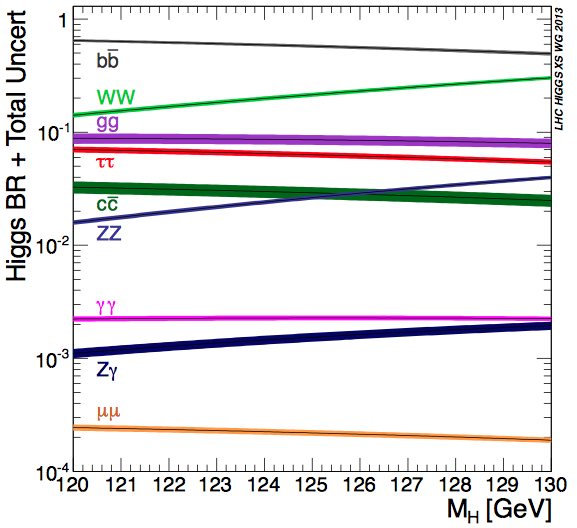
\includegraphics[scale=0.5]{figures/Decays.png}
\caption{Main decays of Higgs bosons branching ratios. Total theoretical uncertainties shown. All credits to \copyright PDG.}
\label{fig:decays}
\end{figure}

Each channel has different challenges associated with tagging it as a Higgs event. The $H->b\bar{b}$decay mode is of a particular challenge even with it's large BR. The problem comes from the huge multijet (MJ) background which we must be able to cut\cite{higgsBB}. To get a clean signature for triggering the decay $H->b\bar{b}$ in association with a Z/W boson is searched for. The leptonic decay channels can use muon or electron triggers to differentiate between signal and background. Furthermore missing $E_t$ can be used to trigger the ZH->$\nu\nu b\bar{b}$ channel. This signature still has many background processes that can be confused for signal. The main background come from (W/Z)+jets and $t\bar{t}$ production with smaller contributions made from single top and diboson production. To remove these backgrounds other discriminating variables must be used. The invariant mass of the dijet system, internal and distributive characteristics of the jets and b-tagging are some of the variable with the most discriminating power. Determining all the variables and values of there cuts depends on many factors and must be investigated for each new analysis.           


